% reducesymm/linresp/McICvi15.tex
% $Author: predrag $ $Date: 2015-10-14 00:30:40 -0400 (Wed, 14 Oct 2015) $

                        %% logical setup, no need to edit %%%%%%%%%%
                        \newif\ifpaper \newif\ifPDF               %%
                        \newif\ifOUP \newif\ifboyscout            %%
                        \newif\ifdasbuch \newif\ifarticle         %%
                        \newif\ifsolutions

                        \newif\ifboyscout                         %%
                        \boyscouttrue %% commented, WWW/boyscouts %%
                        \newif\ifpreparepdf                       %%
                        \preparepdftrue % hyperlinked pdf default %%

    % Toggle between draft and non-draft versions
%  \boyscoutfalse                 % public, hyperlinked
%  \preparepdffalse\boyscoutfalse % public, B&W print version

%                    PRE resubmission:
%                    arXiv submission:
%                    finished editing:
% Note: {revtex4} has been replaced by {revtex4-1} by APS
%       revert to {revtex4} if you have an old configuration
%       read also sliceDefs.tex
%                    finished writing:
%                    PRE submission:
%                    arXiv submission: =
% Predrag 2nd rewrite
%                    finished writing: Predrag
% Predrag completed rewrite
% Predrag
%%                   started writing:  Predrag
% Benjamin    1. draft stoch.tex


%% ------------------ for arXiv submission ----------------------------
%
% Title:    Periodic Orbit Theory of Linear Response
% Authors:  Benjamin McInroe and Predrag Cvitanovic
% Comments: ? pages, ? pdf figures, uses revtex4
% Files:    McICvi15.tex sliceDefs.tex slice.bbl
%           fig??.pdf fig??.pdf
%
%% ------------------ cut here ----------------------------------------



%        \ifboyscout
%\documentclass[pre,aps,twocolumn,showpacs,hyperref]{revtex4-1} %or {revtex4-1}
%        \else
%\documentclass[pre,aps,twocolumn,showpacs,superscriptaddress]{revtex4} %or {revtex4-1}
%\documentclass[prl,aps,preprint,showpacs]{revtex4-1} %or {revtex4-1}
%        \fi

\documentclass[twocolumn,aip,cha]{revtex4-1}
\usepackage{graphicx}% Include figure files

\begin{document}
\title{Periodic Orbit Theory of Linear Response}
\author{Benjamin McInroe}
\affiliation{School of Physics, Georgia Institute of Technology, Atlanta, Georgia 30332, USA}
\author{Predrag Cvitanovic}
\affiliation{School of Physics, Georgia Institute of Technology, Atlanta, Georgia 30332, USA}

\date{\today}

\begin{abstract}

This project is an update of previous work by Sondergaard and Cvitanovic (1995). We apply periodic orbit theory to dynamical systems of the form $\frac{dx_{i}}{dt}+\epsilon \delta v_{i}(x), \epsilon \ll 1$, where $\delta v_{i}(x)$ is a spatial perturbation to the flow. Such a perturbation results in a small shift of the eigenvalue spectrum of the evolution operator of the dynamical system, which to linear order for structurally stable dynamics can be computed in terms of the cycle expansion of the flow. Assuming the perturbations to the local traces vary smoothly with the parameter $\epsilon$, the variation of the weighted average of a given observable with respect to $\epsilon$ can also be computed. We apply this formalism to computation of the leading eigenvalues of two one-dimensional maps, the tent map and the logistic map, to demonstrate the results for both a structurally stable and structurally unstable case, respectively. Finally, we apply the formalism to computation of a 'real' observable, the Lyapunov exponent.

\end{abstract}

\maketitle



\section{Introduction}

In this project, we consider the dynamics of weakly perturbed systems of the form $\frac{dx_{i}}{dt}=v_{i}(x) + \epsilon \delta v_{i}(x)$. The study of such systems is relevant to the statistical mechanics of nonequilibrium systems, in which the perturbation might signify an external force that driving the system away from equilibrium. The parameter $\epsilon$ is taken to be sufficiently small such that the perturbing flow may be approximated to linear order, and the well-established approach to problems of this nature has come to be called linear response theory (for a review, see ref). We consider an alternative approach to linear response problems, employing the periodic orbit theory (for example, see (ref 2)) to make predictions for average values of observables.  Section II is an overview of periodic orbit theory used in developing the linear response formalism in Section III. In Section IV, the linear response theory is applied to computations of eigenvalues for one dimensional maps. In Section V and VI, we expand these results to computation of the Lyapunov exponent of these maps, comparing to a recent 'classical' computation by Abramov. [cite]

\section{A Brief Review of Cycling}
This section contains an overview of concepts from periodic orbit theory used in this study. For a more thorough introduction, 'chaosbook' is strongly recommended.
\subsection{Zeta Functions, Cycle Expansions, and All That}
Consider a dynamical system given by a measure preserving flow, $f: M\rightarrow M$, where $M$ is a locally Euclidean manifold, the state space. If the dynamical system is chaotic, then it is impossible to compute asymptotic trajectories for a single initial point in $M$. But all is not lost, and we can trade the notion of a single initial point, $x_{0}\in M$, evolved forward in time by the flow $f$, for an initial 'density' of points, $\rho (x, 0), x\in M$, evolved forward in time by an evolution operator, $L^{t}$.
\indent Our ultimate goal is the computation of average values of observables for the system $(M, f)$, and thus we turn our attention to the spectrum of the evolution operator. Our method of choice here is by construction of the dynamical zeta function, which has the Euler product form,
\begin{equation}
\frac{1}{\zeta} = \prod_{p} (1 - t_{p})
\end{equation}
where $t_{p}$ is the weight associated with the prime cycle p. The eigenvalues of the evolution operator are then given by the zeros of the dynamical zeta function, that is,
\begin{equation}
\frac{1}{\zeta (s_{\alpha})} = 0
\end{equation}
For the $\alpha^{th}$ eigenvalue, $s_{\alpha}$. To compute the zeros, consider the expansion of the zeta function in a formal power series,
\begin{equation}
\frac{1}{\zeta} = 1 - \sum_{p_{1}+p_{2}+...p_{k}}^{'}t_{p_{1}+p_{2}+...p_{k}}
\end{equation}
for $t_{p_{1}+p_{2}+...p_{k}} = (-1)^{k+1}t_{p_{1}}t_{p_{2}}...t_{p_{k}}$, where the prime on the sum indicates that the sum is taken over all distinct, non-repeating combinations of prime cycles. When $k>1$, $t_{p_{1}+p_{2}+...p_{k}}$ are weights of pseudocycles, sequences of shorter cycles the shadow a cycle with symbol sequence $p_{1}p_{2}...p_{k}$, along the segments $p_{1}, p_{2}, ..., p_{k}$. This series representation of a dynamical zeta function or spectral determinant is known as the cycle expansion. It is a sum over pseudocycles, ordered by increasing cycle length and instability.

\indent Now comes the key step. The cycle expansion for a dynamical system with finite grammar may be regrouped into sums of fundamental contributions, $t_{f}$, and decreasing curvature contributions, $c_{n}$. That is,
\begin{equation}
\frac{1}{\zeta} = 1 - \sum_{f}t_{f} - \sum_{n}c_{n}
\end{equation}
where the fundamental contributions $t_{f}$ are cycles with no shorter approximants. They are the 'building blocks' of the dynamics, from which longer orbits may be approximately pieced together. The curvature contributions $c_{n}$ are the longer orbits pieced together from fundamental contributions, and their shadowing approximants. For continuous and smooth flows, orbits of similar symbolic dynamics will traverse the same neighborhoods, and have similar weights. The result is that for such flows, the curvature contributions to the cycle expansion will almost cancel. The utility of cycle expansions is now clear: by grouping the terms, we find that the cycle expansion is dominated by the short cycles, with long cycles giving exponentially decaying corrections. The cycle expansion for binary symbolic dynamics is computed in Appendix A.
\subsection{Averaging for Cyclists}
We now use the formalism of the previous section to compute averages of observables. Consider the weight for the cycle $p$,
\begin{equation}
t_{p} = t_{p}(\beta, s(\beta)) = \frac{1}{\mid \Lambda_{p} \mid} e^{\beta A_{p} - s(\beta)T_{p}}
\end{equation}
where $\Lambda_{p}$ is the Floquet multiplier, $A_{p}$ is an observable of interest, and $T_{p}$ is cycle period (or topological cycle length for discrete dynamics). With this weight, (2) is now an implicit equation for $s=s(\beta)$, for arbitrary parameter $\beta$, of the form $G(\beta, s(\beta)) = 0$. The cycle averaging formulas for the slope and curvature of $s(\beta)$ follow from differentiation of the eigenvalue condition with respect to $\beta$,
\begin{eqnarray*}
0 = \frac{d G}{d\beta} = \frac{\partial G}{\partial \beta} + \frac{\partial s}{\partial \beta}\frac{\partial G}{\partial s}
\\ \Rightarrow \frac{\partial s}{\partial \beta} = -\frac{\partial_{\beta}G}{\partial_{s} G}
\end{eqnarray*}
Denoting by,
\begin{eqnarray*}
&\langle A\rangle_{G}& = -\frac{\partial G}{\partial \beta}\mid_{\beta, s=s(\beta)},\\ &\langle T \rangle_{G}& = \frac{\partial G}{\partial s}\vert_{\beta, s=s(\beta)}
\end{eqnarray*}
respectively the mean cycle expectation value of $A$ and the mean cycle period, both weighted by $G$. The cycle averaging formula for the expectation value of the observable is then,
\begin{equation}
\langle a\rangle = \frac{\langle A \rangle_{G}}{\langle T \rangle_{G}}
\end{equation}
For $G = 1/\zeta$, we obtain the zeta - weighted average formulas. Using the cycle expansion representation,
\begin{eqnarray*}
&\langle A \rangle_{\zeta}&:=-\frac{\partial}{\partial \beta}\frac{1}{\zeta}=\sum^{'}(A_{p_{1}}+A_{p_{2}}+...+A_{p_{k}})t_{p_{1}+p_{2}+...+p_{k}} \\
&\langle T \rangle_{\zeta}&:=\frac{\partial}{\partial s}\frac{1}{\zeta}=\sum^{'}(T_{p_{1}}+T_{p_{2}}+...+T_{p_{k}})t_{p_{1}+p_{2}+...+p_{k}}
\end{eqnarray*}
These are the dynamical zeta function averages over prime cycles, with cycle weights evaluated at leading eigenvalues $t_{p} = t_{p}(\beta,s(\beta))$. For bounded flow, $s(0)=0$, so
\begin{eqnarray*}
&\langle A \rangle_{\zeta}& = \sum^{'}(-1)^{k+1}\frac{A_{p_{1}}+A_{p_{2}}+...+A_{p_{k}}}{\vert \Lambda_{p_{1}}...\Lambda_{p_{k}}\vert}\\
&\langle T \rangle_{\zeta}& = \sum^{'}(-1)^{k+1}\frac{T_{p_{1}}+T_{p_{2}}+...+T_{p_{k}}}{\vert \Lambda_{p_{1}}...\Lambda_{p_{k}}\vert}
\end{eqnarray*}
As before, these cycle expansions are grouped as fundamental and curvature terms, with nearby pseudoorbits nearly vanishing. All zeta weighted averages in this paper are weighted with (5). The cycle expansion averages are worked out explicitly for binary symbolic dynamics in Appendix A.

\section{Linear Response in terms of periodic orbits}

In section A, we discuss the theoretical formalism for the periodic orbit theory approach to linear response. In section B, we use the one dimensional unimodal tent map as a simple, exactly solvable example of the technique, and as a prelude to the continuous time case.

\subsection{Eigenvalue shift using dynamical zeta function}

Consider a dynamical system of the form,
\begin{equation}
\frac{dx_{i}}{dt}=v_{i}(x)
\end{equation}
The eigenvalues of the evolution operator of (7), $s_{\alpha}$, satisfy the condition on the dynamical zeta function (2),
\begin{equation}
\frac{1}{\zeta_{0} (s)} = 0
\end{equation}
Under a small perturbation to the flow, $\epsilon \delta v_{i}(x)$, the system becomes,
\begin{equation}
\frac{dx_{i}}{dt}=v_{i}(x) + \epsilon \delta v_{i}(x), \vert\epsilon\vert \ll 1
\end{equation}
The result of such a perturbation is a small shift in the eigenvalues of the evolution operator, such that $s_{\alpha}\rightarrow s_{\alpha} + \delta s_{\alpha}$. Then the new condition on the dynamical zeta function is,
\begin{equation}
\frac{1}{\zeta(s_{\alpha}+\delta s_{\alpha})} = 0
\end{equation}
which can be expanded to linear order and solved for $\delta s_{\alpha}$ as,
\begin{equation}
\delta s_{\alpha} = -\frac{1/\zeta(s_{\alpha})}{\frac{\partial}{\partial s}\zeta (s_{\alpha})}
\end{equation}
The cycle expansion of $1/\zeta(s)$ is a cycle by cycle deformation of $\frac{1}{\zeta_{0}}(s)\pm$ new / lost cycles. For structurally stable dynamics, we can ignore the possibility of gaining or losing new cycles, and expand the numerator of (11) to linear order as,
\begin{equation}
\frac{1}{\zeta (s_{\alpha})} = \sum_{p}t_{p}(s_{\alpha}) + \sum_{p}\delta t_{p}(s_{\alpha})
\end{equation}
The first term is the cycle expansion of the zeta function (II.A), and is zero by (8). The denominator of (11) may be evaluated by noting that to leading order, $1/\zeta(s_{\alpha}) \cong 1/\zeta_{0}(s_{\alpha})$, then from (II.B),
\begin{eqnarray*}
\frac{\partial}{\partial s}\frac{1}{\zeta (s_{\alpha})} = \frac{\partial}{\partial s}\frac{1}{\zeta_{0} (s_{\alpha})} = \sum_{p}\frac{\partial}{\partial s}t_{p}(s_{\alpha}) \\ =  \sum_{p}T_{p}t_{p}(s_{\alpha}) =  \langle T_{p}\rangle_{\zeta}
\end{eqnarray*}
The numerator may be evaluated by expanding $\delta t_{p}$ in terms of variations of $A_{p}$, $T_{p}$, and $\Lambda_{p}$. Substituting for (11), we find,
\begin{equation}
\delta s_{\alpha} = -\frac{\beta \langle\delta A_{p}\rangle_\zeta - s\langle\delta T_{p}\rangle_{\zeta} - \langle\frac{\delta \Lambda_{p}}{\Lambda_{p}}\rangle_{\zeta}}{\langle T\rangle_{\zeta}}\vert_{s=s_{\alpha}}
\end{equation}
which is the expression for the shift of the perturbed eigenvalues.

\subsection{Cycle averaging formulas for linear response of observables}
We have found that for structurally stable, hyperbolic dynamics, the eigenvalue $s_{\alpha}$ and the characteristics of the orbits depend on the variation parameter of the system, $\epsilon$. However, for each fixed value of $\epsilon$, the cycle averaging formula should be applicable, thus,
\begin{eqnarray}
\frac{\partial \langle a\rangle_{\zeta}}{\partial \epsilon} = \frac{\partial}{\partial \epsilon}\frac{\langle A \rangle_{\zeta}}{\langle T \rangle_{\zeta}} =
\frac{\frac{\partial \langle A \rangle_{\zeta}}{\partial \epsilon} - \langle a \rangle_{\zeta}\frac{\partial \langle T \rangle_{\zeta}}{\partial \epsilon}}{\langle T \rangle_{\zeta}}
\end{eqnarray}
where we have simplified the final expression with (6).

\indent We remark that in a typical calculation of a physical average, $\beta$ is put to zero. For a bounded system the leading eigenvalue $s_{0}=0$, is independent of the perturbation. In Appendix (14), we evaluate (14) step-by-step. The result is,
\begin{eqnarray*}
&\frac{\partial \langle a\rangle_{\zeta}}{\partial \epsilon}& = \frac{1}{\langle T \rangle_{\zeta}}\Bigg( \left\langle (\beta(A-\langle a\rangle T + 1)\frac{\partial A}{\partial \epsilon}\right\rangle \\ &-& \left\langle (s_{\alpha}-(1-s_{\alpha})\langle a\rangle)\frac{\partial T}{\partial \epsilon}\right\rangle  \\
&-&\left\langle (A-\langle a \rangle T) \frac{\frac{\partial \Lambda}{\partial \epsilon}}{\Lambda}\right\rangle \Bigg)
\end{eqnarray*}
This completes the analysis of periodic orbit theory of linear response.

\section{Results of analytic and numerical tests}
subsection{Tent Map}
As a simple, one dimensional discrete example to provide insight into the application of the formalism established in the previous section, we consider the tent map, of the form,
\begin{equation}
f(x) = \left\{
     \begin{array}{lr}
       \Lambda_{0} x & : x \in M_{0}\\
       \Lambda_{1} (1-x) & : x \in M_{1}
     \end{array}
   \right.
\end{equation}
Where the two state space regions, $M_{0}$ and $M_{1}$, are partitioned by the critical point at which the two sides of the map are equal. This type of unimodal map is particularly desirable, as its evolution operator has a simple, finite dimensional form (see Ref). As a result, the leading eigenvalue $s_{0}$ may be written analytically as
\begin{equation}
s_{0} = ln\left( \frac{1}{\mid \Lambda_{0}\mid}+\frac{1}{\mid \Lambda_{0}\mid}\right)
\end{equation}
where $\mid \Lambda_{i} \mid$ are the slopes of the left and right sides of the map. [Fig. 1]


\begin{figure}[t]
\begin{centering}
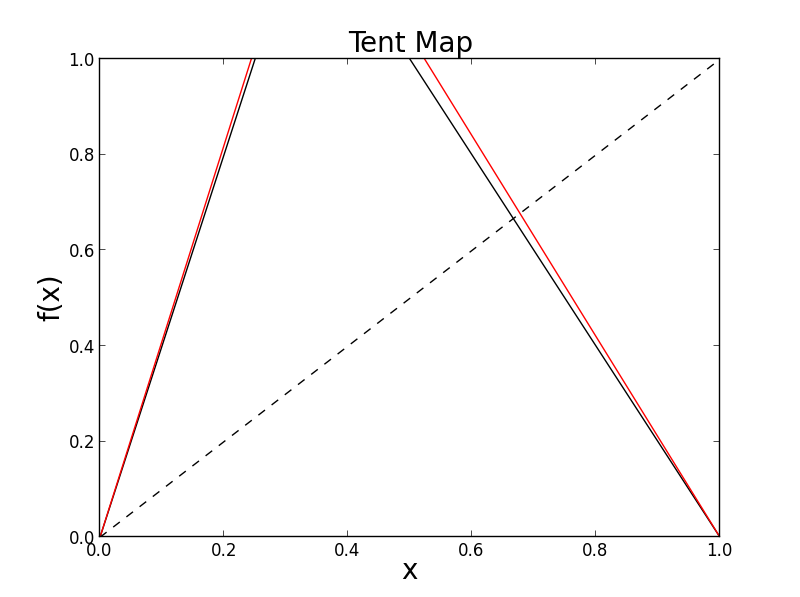
\includegraphics[scale=.4]{tent map example.png}

\caption{An example plot of the tent map repeller. The black lines correspond to the unperturbed tent map with $\mid \Lambda_{0}\mid=4$, $\mid \Lambda_{1}\mid=6$. The red lines correspond to a possible perturbed tent map, with perturbation...}

\end{centering}
\end{figure}

\indent Consider a perturbation to the tent map that slightly shifts the slopes of the two sides. That is, a perturbation of the form,
\begin{equation}
f(x) = \left\{
     \begin{array}{lr}
       \Lambda_{0} x+\epsilon x & : x \in M_{0}\\
       \Lambda_{1} (1-x)-\epsilon x & : x \in M_{1}
     \end{array}
   \right.
\end{equation}
for $\mid \epsilon \mid \ll 1$. The example for $\mid \epsilon \mid = 0.1$ is plotted in [Fig. 1]. The perturbation is conveniently chosen such that it shifts the values of the Floquet multipliers by $+\epsilon$, and the leading eigenvalue can be computed exactly from (16). Using the periodic orbit theory approach from III.A, the approximate shift of the leading eigenvalue can be computed from (13). Taking $\beta=0$, and noting that for the example in [Fig. 1], with $\epsilon\in [0,1]$, the perturbation does not change the symbolic dynamics, so that the second term in the numerator also vanishes,

\begin{equation}
\delta s_{\alpha} = \frac{1}{\langle T \rangle}_{\zeta} \left\langle \frac{\delta \Lambda_{p}}{\Lambda_{p}} \right\rangle_{\zeta}
\end{equation}

The computation is straightforward for binary symbolic dynamics, and may be found in Appendix A. A comparison of the exact and linear response results is plotted in [Fig. 2]. In particular, curvature terms are neglected when computing the cycle averages used in [Fig. 2] in order to simplify computations.


\begin{figure}[t]
\begin{centering}
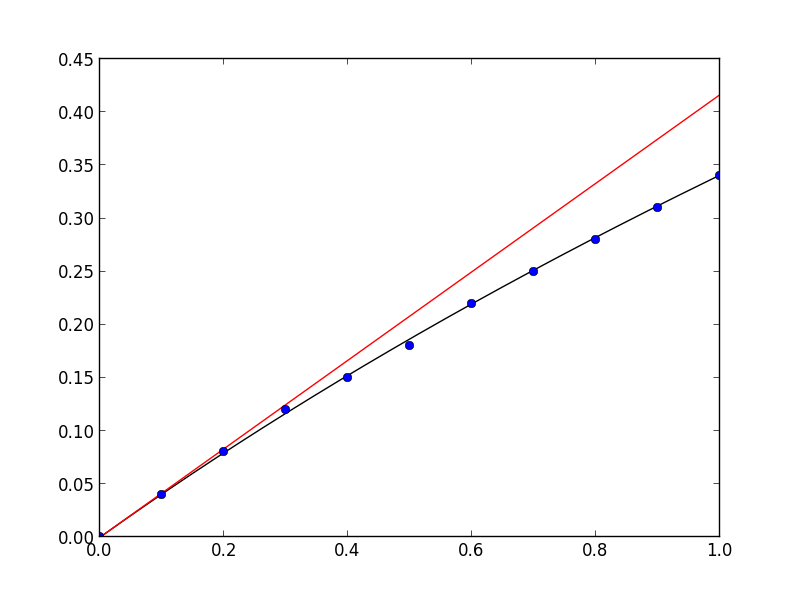
\includegraphics[scale=.4]{numeric.png}

\caption{Results of the tent map repeller exact (black), linear response (red), and numerical (blue points) calculations of eigenvalue shift for the map in [Fig. 1]. For $\epsilon$ sufficiently small, the results agree to high precision. The numerical calculation is done for the physical interpretation of the leading eigenvalue as the escape rate of the repeller, $\gamma = -s_{0}$.}

\end{centering}
\end{figure}
\subsection{Logistic Map}
In III.A, we made the assumption that the dynamics of the perturbed system are structurally stable, that is, the perturbing flow does not create or destroy fixed points or periodic orbits. What if we were to choose a case for which this is not true? Would the linear response theory still provide a good approximation for the eigenvalue shift? To help answer these questions, we start by considering one of the simplest nonlinear maps with chaotic properties, the logistic map,
\begin{equation}
f(x) = rx(1 - x), x\in [0, 1]
\end{equation}
for which a small perturbation to the parameter r can result in a period doubling bifurcation. We consider a perturbation of the form,
\begin{equation}
\epsilon \delta f(x) = \epsilon x(1-x), \mid \epsilon \mid \ll 1
\end{equation}
The symbolic dynamics are again binary, so computation of the actual eigenvalues is done as in the previous section.

\begin{figure}[t]
\begin{centering}
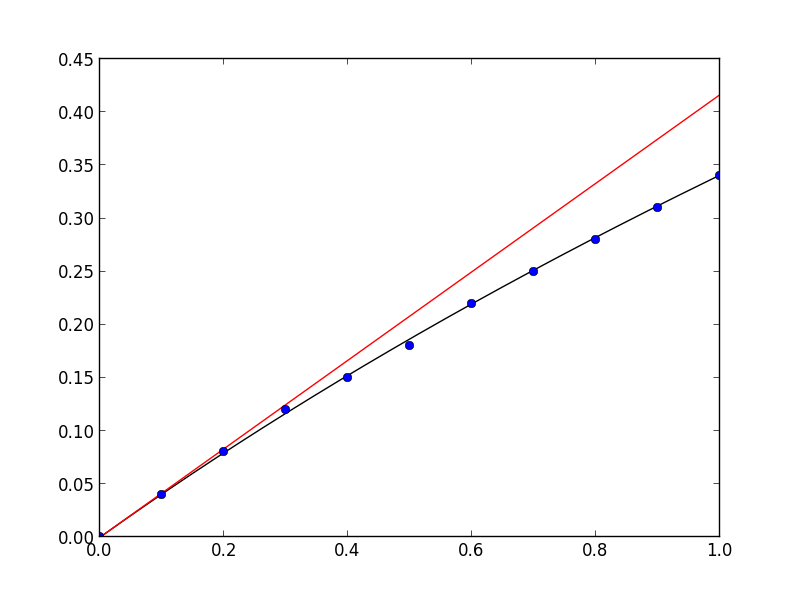
\includegraphics[scale=.4]{numeric.png}

\caption{Results of the logistic map exact (black), linear response (red), and numerical (blue points) calculations of eigenvalue shift for logistic map (19), with unperturbed $r=3.0$. There is no value of $\epsilon$ for which the linear approximation is close to the actual eigenvalue shift.}

\end{centering}
\end{figure}

\section{Calculation of Lyapunov Exponent}
We now turn our attention to the calculation of a 'real' observable for the perturbed maps, the Lyapunov exponent. The Lyapunov exponent is sometimes considered to be an indicator of a chaotic dynamical system, with chaotic dynamics having a positive Lyapunov exponent, corresponding to exponential divergence of flows for nearby initial conditions.

\subsection{Derivation of Lyapunov Exponent}
Let $\bf x(t)$ be an orbit of the set of differential equations (7) with initial state $\bf x_{0}$, that is, $\textbf{x(t)} = f^{t}(\textbf{$\bf x_0$})$, where $f^t$ is the flow of (7). For a small perturbation to this initial state, $\bf \delta x_{0}$, we have another orbit, $\textbf{x(t)} + \textbf{$\bf \delta x(t)$}$ = $f^{t}(\textbf{$\bf x_{0}$} + \textbf{$\bf \delta x_{0}$})$. As our ansatz, suppose that as the orbits evolve, the separation $\bf \delta x_{0}$ grows as,

\begin{equation}
e^{\lambda t} \approx \left\Vert \frac{\bf \delta x(t)}{\bf \delta x_{0}} \right\Vert
\end{equation}

Rearranging, this expression becomes exact in the limit,

\begin{equation}
\lambda = lim_{t\rightarrow \inf} \frac{1}{t} \sum_{i} t_{i} \lambda_{i}
\end{equation}

Where $t = \sum_{i} t_{i}$. In practice, one would let the separation grow until $\Vert \bf \delta x(t_{1}) \Vert$ is sufficiently large (at time $t_{i}$), record the value of the Lyapunov exponent, re-scale back to the linear regime, and continue ad infinitum.
\indent If we let the initial separation tend to zero, then,

\begin{equation}
lim_{\bf \delta x_{0} \rightarrow 0} \frac{\bf \delta x(t)}{\bf \delta x_{0}} = \frac{\bf \partial x(t)}{\bf \partial x_{0}} = J^{t}(\bf x_{0})
\end{equation}

Where $J^{t}$ is the Jacobian matrix of the flow at time $t$. It follows then that the leading Lyapunov exponent is,

\begin{equation}
\lambda(\textbf{$x_{0}$}) = lim_{t\rightarrow \inf}\frac{1}{t} ln \frac{\Vert J^{t}(\textbf{$x_{0}$}) \textbf{$\delta x_{0}$} \Vert}{\Vert \textbf{$\delta x_{0}$} \Vert}
\end{equation}

\subsection{Linear Response for Lyapunov Exponent - Classical Formulation}

\subsection{Linear Response for Lyapunov Exponent - Cyclist's Formulation}
\section{Conclusions}
We developed the periodic orbit formalism for the computation of the linear response of eigenvalues for a general, N dimensional system of differential equations. Furthermore, we applied our result to the calculation of the shift in the eigenvalue spectrum of one dimensional maps with both a hyperbolic and non-hyperbolic fixed point. As expected, while the periodic orbit theory result for the shift in the eigenvalue spectrum was valid for small perturbations in the hyperbolic case, the approximation broke down in the non-hyperbolic case, yielding incorrect results for even the zero perturbation case. Specifically, there is no reason to assume that cycle-expansion parameters vary continuously with respect to the perturbation parameter in the non hyperbolic case, rendering the formalism we developed in Sec. III useless for such cases.
\indent In Sec. V, we showed the utility of the periodic orbit approach for calculating the linear response of the Liapunov exponent of the one dimensional maps from before. We recover the result from Abramov's calculation, but exchange integrals over long trajectories for finite sums over a few prime cycles.

\indent A natural expansion of this work would be to compute observables for a higher dimensional system, in which case the utility of the periodic orbit approach will be even more obvious.
\newpage
\section{Appendix}
\subsection{Cycle Expansion for Binary Symbolic Dynamics}
The simplest example of the cycle expansion is that for the binary symbolic dynamics, of interest when the state space $M$ may be partitioned into two regions, labeled $M_{0}$ and $M_{1}$. The Euler product representation of the dynamical zeta function is then,
\begin{eqnarray*}
\frac{1}{\zeta} &=& (1 - t_{0})(1-t_{1})(1-t_{01})(1-t_{001})(1-t_{011})
\\ &(1-t_{0001})&(1-t_{0011})(1-t_{0111})...
\end{eqnarray*}
for cycles up to topological length four. Expanding the product, we obtain the cycle expansion form of the zeta function,
\begin{eqnarray*}
\frac{1}{\zeta} &=& 1 - t_{0} - t_{1} - t_{001} - t_{011} - t_{0001} - t_{0011} - t_{0111} - ...
\\ &-& t_{0+1} - t_{01+1} - t_{0+001} - t_{0+011} - ...
\end{eqnarray*}
Next, we regroup the terms in the above expansion into fundamental and curvature contributions. In this example, there are only two fundamental contributions to the cycle expansion, corresponding to the $M_{0}$ and $M_{1}$ fixed points,
\begin{eqnarray*}
\frac{1}{\zeta} &=& 1 - t_{0} - t_{1} \\ &-& [(t_{01} - t_{1}t_{0})] \\ &-& [(t_{001} - t_{01}t_{0}) + (t_{011} - t_{01}t_{1})] - ...
\end{eqnarray*}
As expected, the curvature terms nearly cancel, leaving the fundamental contributions as the dominant terms in the series, a result used to simplify computations of averages in Sec. IV. For example, for the average cycle period, the cycle expansion with the usual weight is,
\begin{eqnarray*}
\langle T \rangle_{\zeta} &=& \frac{T_{0}}{\Lambda_{0}} + \frac{T_{1}}{\Lambda_{1}} + \left( \frac{T_{01}}{\Lambda_{01}}-\frac{T_{0} + T_{1}}{\Lambda_{0}\Lambda_{1}}\right)
\\ &+& \left( \frac{T_{001}}{\Lambda_{001}}-\frac{T_{01} + T_{0}}{\Lambda_{01}\Lambda_{0}}\right) +...
\end{eqnarray*}
This is the cycle expansion average calculated in II.B for symbolic dynamics. A similar result is found for the cycle expansion average of $A$.
\subsection{Variation of $\langle a \rangle_{\zeta}$ in $\epsilon$}
Here we derive final equation in III.B for the variation of $\langle a\rangle_{\zeta}$ in the parameter $\epsilon$. We start by computing the variations of the cycle expectation values of $A$ and $T$,
\begin{eqnarray*}
\frac{\partial \langle A \rangle_{\zeta}}{\partial \epsilon} = \frac{\partial}{\partial \epsilon}\sum_{p}t_{p}A_{p} = \sum_{p}\frac{\partial t_{p}}{\partial \epsilon}A_{p} + \sum_{p} \frac{\partial A_{p}}{\partial \epsilon} t_{p}
\\ = \sum_{p}t_{p}\Bigg( \Bigg( -s\frac{\partial T_{p}}{\partial \epsilon} + \beta \frac{\partial A_{p}}{\partial \epsilon} - \frac{\frac{\partial \Lambda_{p}}{\partial \epsilon}}{\Lambda_{p}}\Bigg) A_{p} +\frac{\partial A_{p}}{\partial \epsilon} \Bigg)
\end{eqnarray*}
and for $T$,
\begin{eqnarray*}
\frac{\partial \langle T \rangle_{\zeta}}{\partial \epsilon} = \frac{\partial}{\partial \epsilon}\sum_{p}t_{p}T_{p} = \sum_{p}\frac{\partial t_{p}}{\partial \epsilon}T_{p} + \sum_{p} \frac{\partial T_{p}}{\partial \epsilon} t_{p}
\\ = \sum_{p}t_{p}\Bigg( \Bigg( -s\frac{\partial T_{p}}{\partial \epsilon} + \beta \frac{\partial A_{p}}{\partial \epsilon} - \frac{\frac{\partial \Lambda_{p}}{\partial \epsilon}}{\Lambda_{p}}\Bigg) A_{p} +\frac{\partial T_{p}}{\partial \epsilon} \Bigg)
\end{eqnarray*}
Substituting back into (14), we get,
\begin{eqnarray*}
\frac{\partial \langle a \rangle_{\zeta}}{\partial \epsilon} &=&
\\ \frac{1}{\langle T\rangle_{\zeta}}\Bigg( &\sum_{p}&t_{p}\Bigg( \Bigg( -s\frac{\partial T_{p}}{\partial \epsilon} + \beta \frac{\partial A_{p}}{\partial \epsilon} - \frac{\frac{\partial \Lambda_{p}}{\partial \epsilon}}{\Lambda_{p}}\Bigg) A_{p} +\frac{\partial A_{p}}{\partial \epsilon} \Bigg)
\\ - \langle a \rangle_{\zeta} &\sum_{p}&t_{p}\Bigg( \Bigg( -s\frac{\partial T_{p}}{\partial \epsilon} + \beta \frac{\partial A_{p}}{\partial \epsilon} - \frac{\frac{\partial \Lambda_{p}}{\partial \epsilon}}{\Lambda_{p}}\Bigg) A_{p} +\frac{\partial T_{p}}{\partial \epsilon} \Bigg) \Bigg)
\end{eqnarray*}
Regrouping terms with the same partials, and substituting re-writing the sums  over cycles as cycle average values, we obtain,
\begin{eqnarray*}
&\frac{\partial \langle a\rangle_{\zeta}}{\partial \epsilon}& = \frac{1}{\langle T \rangle_{\zeta}}\Bigg( \left\langle (\beta(A-\langle a\rangle T + 1)\frac{\partial A}{\partial \epsilon}\right\rangle \\ &-& \left\langle (s_{\alpha}-(1-s_{\alpha})\langle a\rangle)\frac{\partial T}{\partial \epsilon}\right\rangle  \\
&-&\left\langle (A-\langle a \rangle T) \frac{\frac{\partial \Lambda}{\partial \epsilon}}{\Lambda}\right\rangle \Bigg)
\end{eqnarray*}
% Make the bibliography from filename Test.bib placed in same directory as Test.tex

\bibliography{lrp}{}


\end{document}
